\documentclass{article}
\usepackage[T1]{fontenc}
\usepackage{lmodern}
\usepackage{graphicx}
\usepackage{amsmath,amssymb}
\usepackage[a4paper,margin=2cm]{geometry}
\usepackage[absolute,overlay]{textpos}
\setlength{\TPHorizModule}{1mm}
\setlength{\TPVertModule}{1mm}
\usepackage[indonesian]{babel}
\usepackage{hyperref}
\setlength{\emergencystretch}{2em}
% unit: Halaman 53

\begin{document}

% === Halaman 53 (llm) ===

\vspace{109.89mm}

\textbf{Triple DES dengan 3 kunci} $(56 + 56 + 56 = 168)$

% deskripsi: Diagram alur proses Enkripsi dan Dekripsi Triple DES dengan 3 kunci berbeda (K1, K2, K3) yang menunjukkan urutan operasi Encrypt (E) dan Decrypt (D).
% bbox normalisasi: [0.0600, 0.1080, 0.9400, 0.9120]
\begin{textblock*}{184.80mm}(12.60mm,32.08mm)
\noindent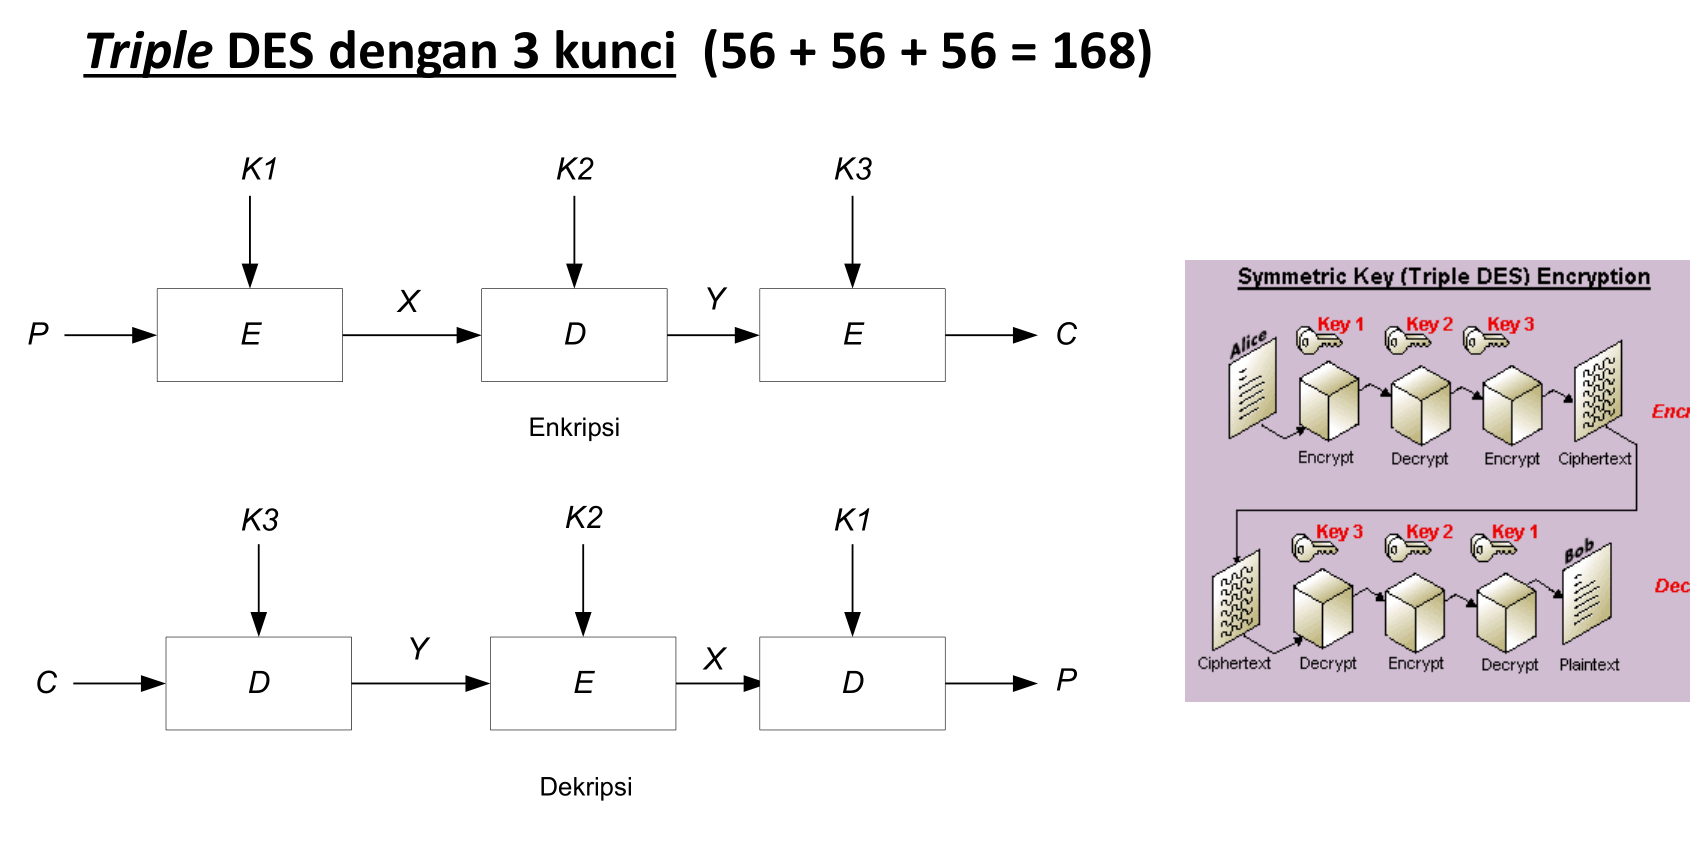
\includegraphics[width=184.80mm,height=238.79mm]{../../images/llm/page_053_img_01.png}%
\end{textblock*}

% deskripsi: Ilustrasi visual enkripsi dan dekripsi simetrik Triple DES yang melibatkan Alice dan Bob, menampilkan penggunaan tiga kunci berbeda dan proses pengubahan Plaintext menjadi Ciphertext dan sebaliknya.
% bbox normalisasi: [0.6800, 0.3100, 0.9800, 0.6800]
\begin{textblock*}{63.00mm}(142.80mm,92.07mm)
\noindent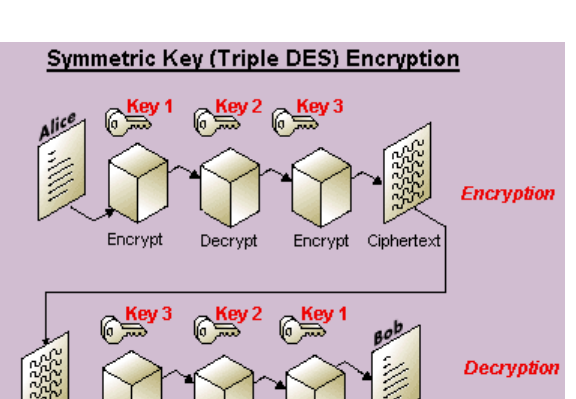
\includegraphics[width=63.00mm,height=109.89mm]{../../images/llm/page_053_img_02.png}%
\end{textblock*}

% bbox perkiraan otomatis: Diagram alur proses Enkripsi dan Dekripsi Triple DES dengan 3 kunci berbeda (K1, K2, K3) yang menunjukkan urutan operasi Encrypt (E) dan Decrypt (D).

\end{document}
